\chapter{Aircraft Design}
\label{ch:aircraftdesign}
\markboth{Aircraft Design}{}

\begin{flushright}
	{\smaller
		\textit{Scientists discover that which exists,\\ engineers creates that which
never was.}\\
		-- T. Von Karman}
\end{flushright}

Engineering design is a non-unique iterative process, the aim of which is to reach the best compromise of a number of conflicting requirements. Whether the need is for a totally new item or for a development of an existing one the design procedure commences with an interpretation of the requirements into a first concept.\\
The conceptual and preliminary design phases play a key role for the best development of future transport aircraft. A software framework that could help in finding a configuration which satisfies several basic requirements and eventually a constrained optimum is an essential tool for academic and industrial aircraft design activity.
Since in the conceptual and preliminary design phases a lot of different configurations have to be analyzed, the software has been conceived to provide results in a relatively short computational time.
For these reasons the the aircraft design is projected to the utilization of new analysis tools who hold a main role in the design and optimization process.\\
Some new software have recently followed innovative approaches considering concepts like KBE (knowledge Based Engineering) and \gls{MDO} (Multi-Disciplinary Optimization) and have highlighted the necessity of an efficient graphical user interface and the importance of making the application results easily exploitable with external software.\\
In this scenery ranks \gls{acr:Adopt} and its reference library \gls{acr:Jpad} that is a Java-based desktop application developed at the University of Naples Federico II, conceived as a fast, reliable and user friendly computational aid for aircraft designers in the conceptual and preliminary design phases.


\section{Historical Overview} 

During the last century, three design methods have been developed in the aerodynamic design process. Until the early 1960s, only two methods were available: empirical and mathematical methods. Since the 1960s, a third method has been developed: computational fluid dynamics, which can be considered as a combination of the two earlier methods. These three methods and their history will be discussed briefly in this chapter. \\
The empirical method  is the oldest method of aerodynamic design; until about 1940, it was the only practical tool available. Based on either theory or experiments or a combination of both, the empirical methods consist of handbooks which are essentially a collection of graphs and equations. They are meant to give a relation between elementary parameters of the geometry of the aircraft and the desired characteristics of the aircraft.\\
Through the mathematical methods the aerodynamic characteristics of the detailed geometry are obtained by physical insight, in other words, through pressure distributions. This approach uses mathematical modelling of flow physics.\\
With the development of computers, more and more powerful numerical methods became available to aircraft designers. These numerical methods are known as computational fluid dynamics. It allows them to obtain the intended characteristics of the aircraft (or one of its major components) by directly determining the required detailed aerodynamic shape through the use of fluid dynamics and the associated pressure distribution.\cite{obert2009aerodynamic}

\noindent \\ \\
Modern aerospace design begins with the desire of mankind to achieve powered, heavier-than-air flight. Early aerospace designs were characterized not only by a great deal of trial and error but also by a not inconsiderable amount of analysis.\\
At the beginning of the aviation history the entire design process occurred in six months. Some companies produced more than ten aircraft in only 20 years. Today in order to develope a new transport aircraft it takes more than 10 years.
The current aircraft design strategy is linked to industrial growth, which in turn depends on national infrastructure, governmental policies, workforce capabilities, and natural resources; these are generally related to global economic–political circumstances. More than any other industry, the aerospace sector is linked to global trends.
It is possible to view the first 75 years of aerospace design as a series of stages: first came the early pioneers, working at a time when many were skeptical about the benefits of flight or even if it was possible at all. Next came the phase where outstanding individuals dominated aeronautical science and design during the interwar and early postwar years. This was followed in the 1950s and 1960s by a greater emphasis on design teams and the massive expansion of the great aerospace companies that we recognize today, such as Lockheed Martin and Rolls-Royce. Following these stages, the advent of CAE, design and manufacture in the mid-1970s transformed activities in aerospace with an increasing focus on faster design cycles, more accurate predictive capabilities and the rise of computer science. At the same time, the great drawing offices of the 1950s declined and fewer people were involved in the design of each individual component.\cite{gambardella}\\
Recent developments in information technology have had a major impact upon the aeronautical design process. The emphasis has become one where the whole design procedure from concept to the derivation of manufacturing data is covered by an integrated information technology system. Computer aided design techniques are used to produce digital data. While these procedures are particularly relevant to the detail phases of the design process their application commences as soon as a requirement is defined and numerical data are derived from it.\cite{howe2000aircraft}


\section{General Process of Aircraft Design}

The design process is usually divided into the following phases:

\begin{enumerate}
\item {\bfseries Requirements phase.}
\item {\bfseries Conceptual design phase.} This phase determines the feasibility of meeting the requirements with a credible aircraft design. The concept definition phase can be characterized as the highly creative and imaginative idea stage during which the component geometry, placement and connectivity of a future aircraft designed to fulfil the needs of a specific market are defined. Conceptual design also entails the development of a novel aircraft concept at an overall system level in competition with a more traditional layout. The objective is to explore a preferred configuration to determine a layout which is technically superior and economically aviable.
\item {\bfseries Preliminary design phase.} This phase aims at defining subsystems and making component trade-offs. Specialists from different functional groups contribute to this process of refining the initial vehicle concept. This team will (re)design the delivered baseline vehicle in suffcient detail to carry out supporting analysis and specify peripheral testing programmes but not with enough detail to specify each sub-assembly.
\item {\bfseries Detail design phase.} In the detail design phase, the confi guration is ``frozen'' and the decision has been made to build the aircraft. Detailed structural design is completed. All of the detail design and shop drawings of the mechanisms, joints, fittings, and attachments are accomplished. Interior layout is detailed with respect to location and mounting of equipment, hydraulic lines, ducting, control cables, and wiring bundles. This development phase is entered soon after the aircraft is committed to production and lasts between two and three years.
\item {\bfseries Testing phase.}
\end{enumerate}

\begin{figure}[H]
\centering
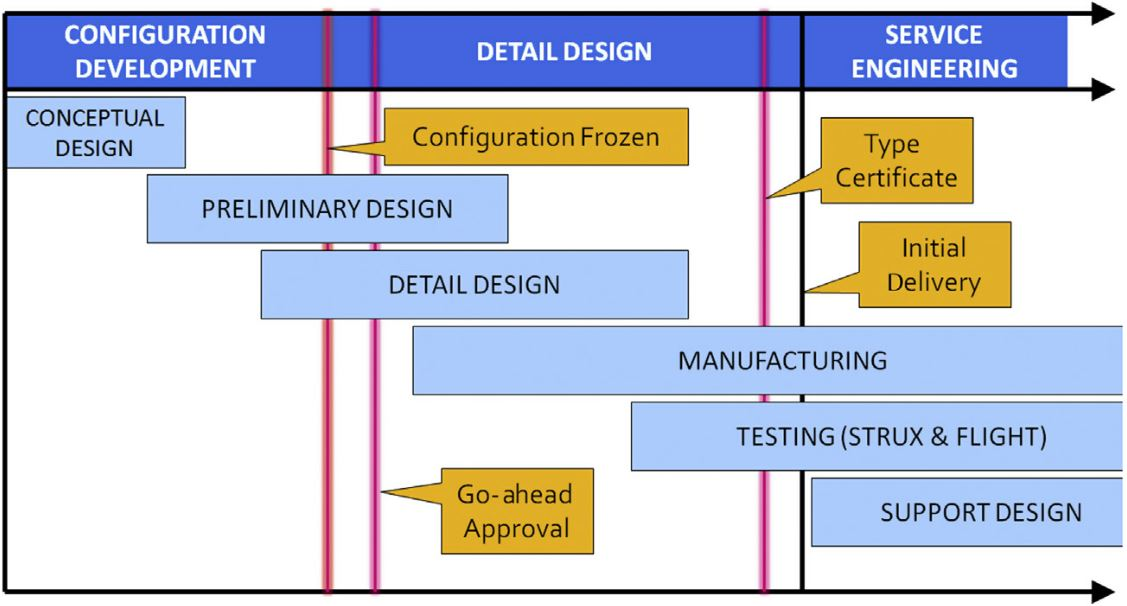
\includegraphics[height = 6 cm ]{Immagini/Process_Design_Torenbeek}
\caption{Aircraft design process for Torenbeek (\num{1986}).}
\label{fig:2}
\end{figure}


\section{Design Requirements and Objectives of an Aircraft}

The general design objective of a transport aircraft is to transport a payload over a distance between airports  against minimum costs (i.e. at an optimum speed).
So, in the design of an aircraft there is never a right answer only a best answer at a point in time. The reason is that the design of an aircraft is a balance between the following competing requirements:

\begin{itemize}
\item {\bfseries Technical.} Performance, survivability
\item {\bfseries Signature.} Survivability, appearance
\item {\bfseries Economic.} Cost, LCC
\item {\bfseries Political.} Policy, payback, risk, and so on
\item {\bfseries Schedule.} When needed? The need to be first to market
\item {\bfseries Environmental.} Limited energy source, noise, hydrocarbon emissions
\end{itemize}

Also, the priorities of these requirements change with time. An aircraft might be designed to certain technical and economic requirements, but if the government administration changes, then the priority requirement becomes political or environmental. The advice to the designer is to remain flexible and develop as robust a design as possible so that it will survive as the requirements change over time. The watchwords are compromise, balance, and flexibility.

\begin{figure}[H]
\centering
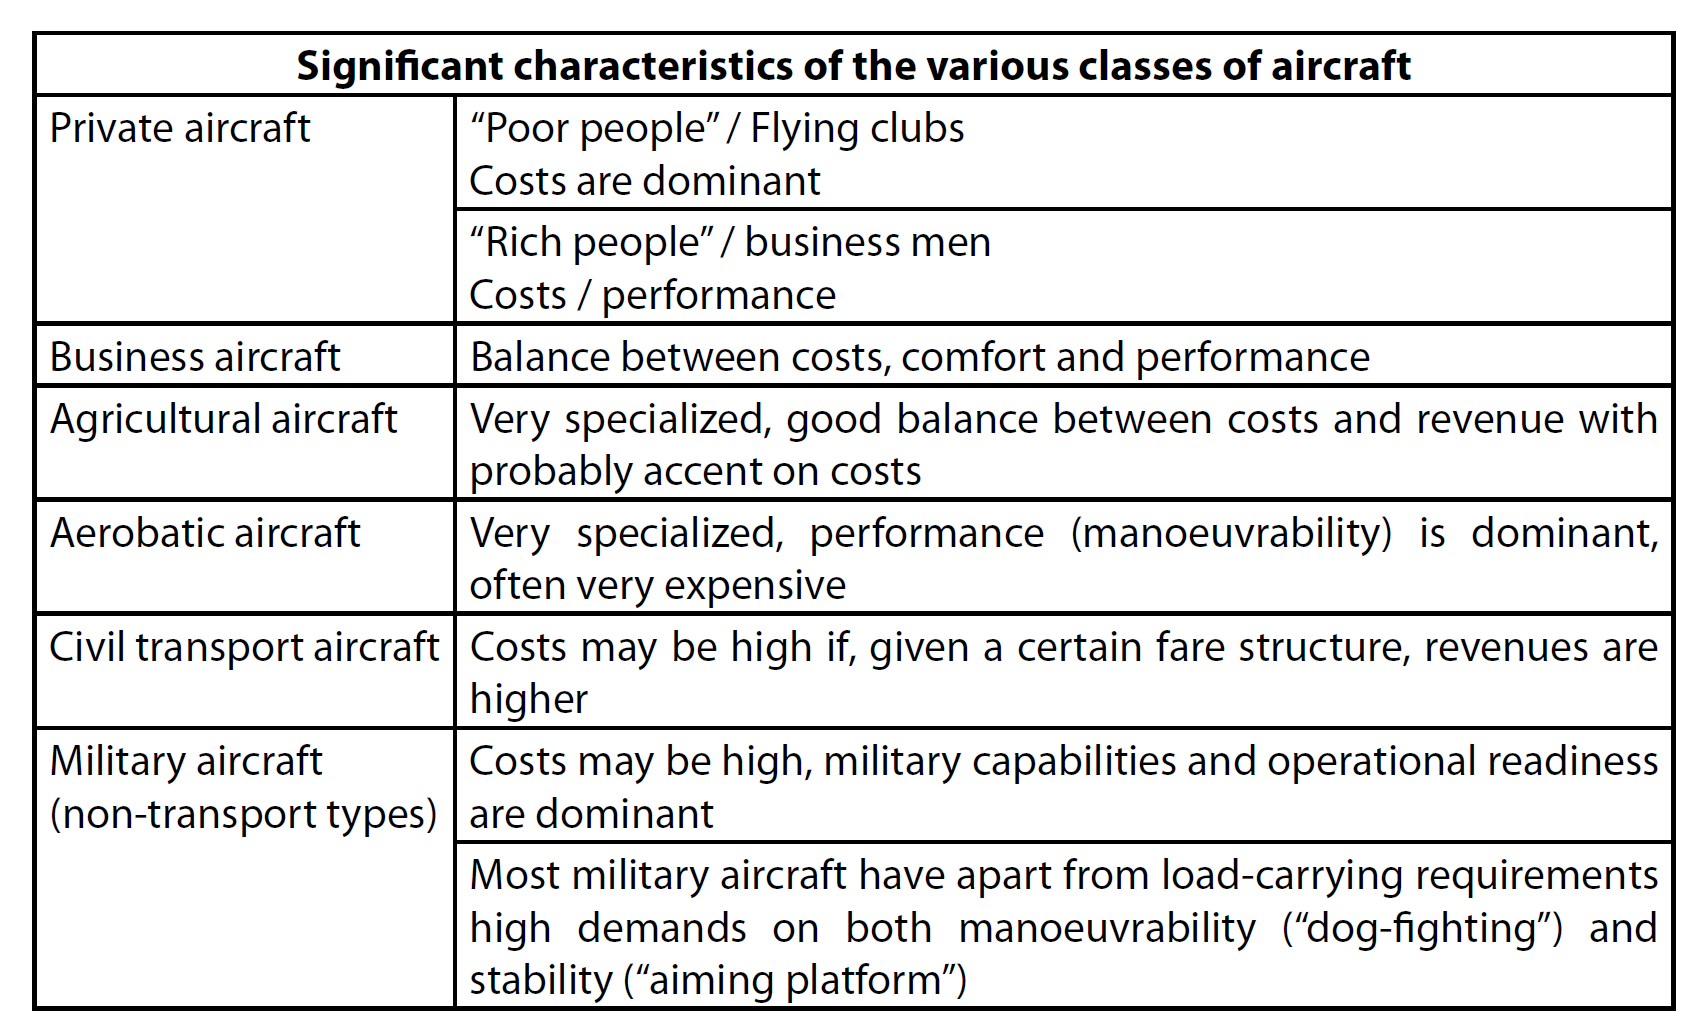
\includegraphics[height=7.9cm]{Immagini/tradeoff}
\caption{Main design requirements of various aircraft categories.\cite{obert2009aerodynamic}}
\label{introduction}
\end{figure}

An aircraft comprised of several major components. It mainly includes wing, horizontal tail, vertical tail, fuselage, propulsion system, landing gear and control surfaces. In order to make a decision about the configuration of each aircraft component, the designer must be fully aware of the function of each component. Each aircraft component has inter-relationships with other
components and interferes with the functions of other components. 

\begin{figure}[H]
\centering
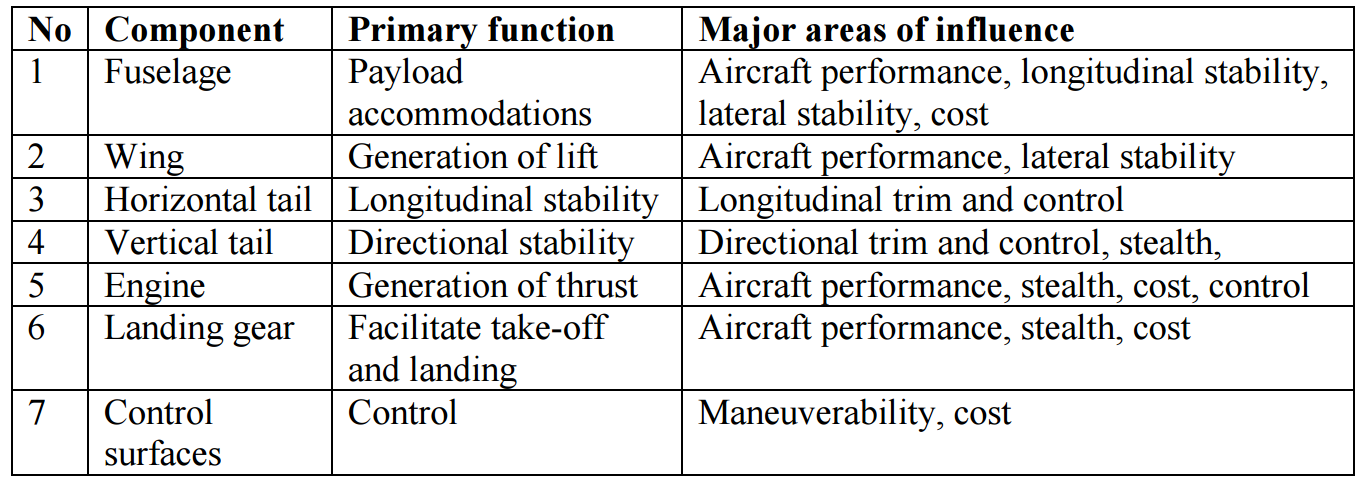
\includegraphics[height=4.9cm]{Immagini/componentfunction}
\caption{Aircraft major components and their functions.\cite{aircraft}}
\label{comp}
\end{figure}

\section{Aircraft Design Optimization}

At the beginning of the aircraft design history, optimization was limited to relatively superficial investigations to study the effects of varying a few major design parameters. 
Since the 1970s, there has been a tremendous expansion of optimization strategies and algorithms supporting advanced designers. The introduction of automated optimization has enabled designers to go into much greater in depth and fidelity of analysis than before. Synthesis programs effectively connecting the inputs and outputs of the functional group disciplines by means of an automatic control logic have been developed at aircraft manufacturers, research establishments and academia. Sophisticated computer assisted design (\gls{acr:cad}) systems for defining three-dimensional body geometries and computer graphics tools for rapidly preparing parametric surveys are available at a modest cost.\\
There are several options available to an aerodynamicist to obtain the best possible solution for a design problem. In general the optimization is an iterative process control system which interprets numerical results and then iteratively assesses variables to seek the global optimum of an objective function. In the aircraft design context, the objective function is used to decide which configuration is considered the best combination of design variables.\cite{torenbeek2013advanced} \\
It is emphasized frequently that optimization of individual goals through separate design considerations may prove counterproductive and usually prevents the overall (i.e., global) optimization of ownership cost.  \gls{MDO} offers good potential but it is not easy to obtain global optimization; it is still evolving. In a way, global  \gls{MDO} involving many variables is still an academic pursuit. Industries are in a position to use sophisticated algorithms in some proven areas. An example is reducing manufacturing costs by reshaping component geometry as a compromise – such as minimizing complex component curvature. The compromises are evident in offering a family of variant aircraft because none of the individuals in the family is optimized, whereas together, they offer the best value.
% continua? 
\noindent \\

\begin{figure}[H]
\centering
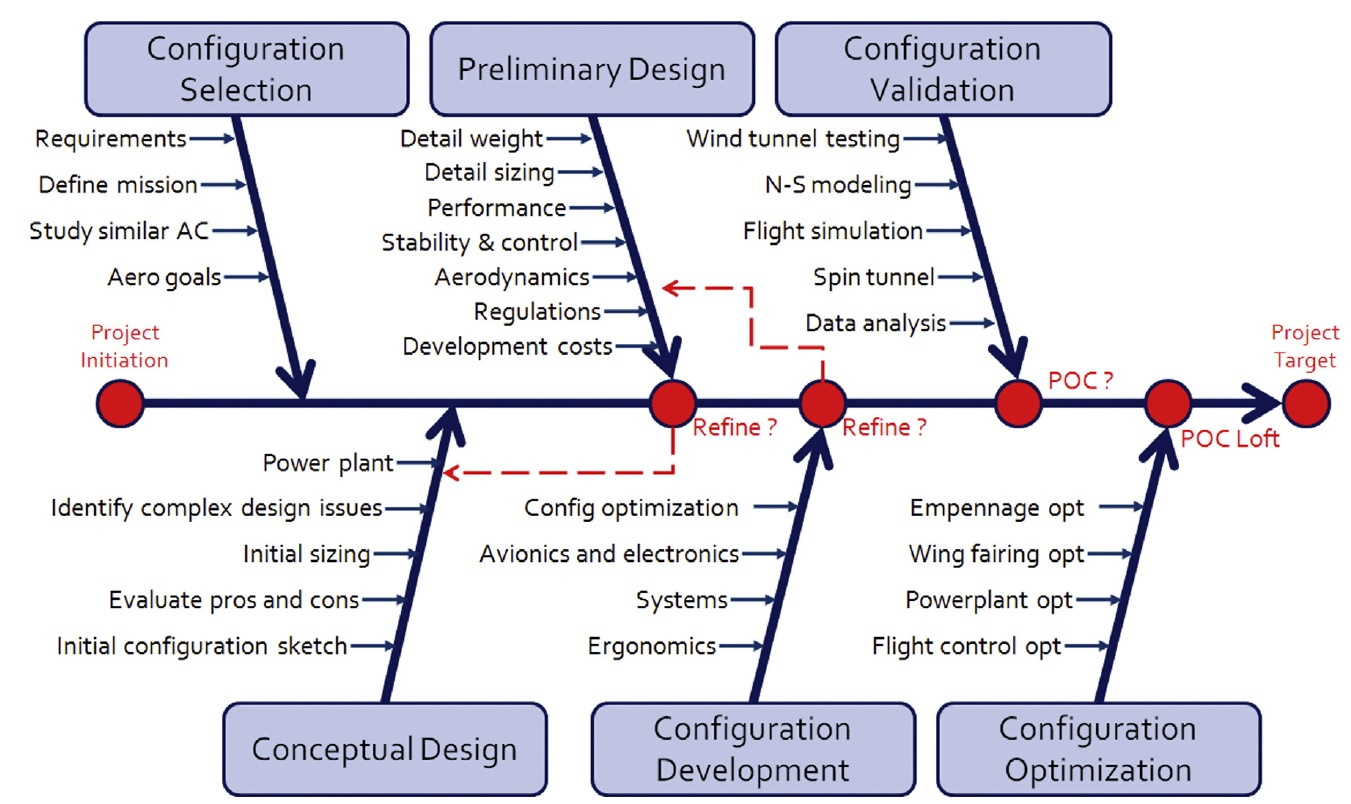
\includegraphics[height=7.6cm]{Immagini/Fishbone}
\caption{A typical fishbone diagram.}
\label{comp}
\end{figure}
